\section{Mutation}\label{mutation}

% http://www.geatbx.com/docu/options-04.html

\paragraph{mutmove}
Beschreibung

\begin{figure}[h!]
  \centering
  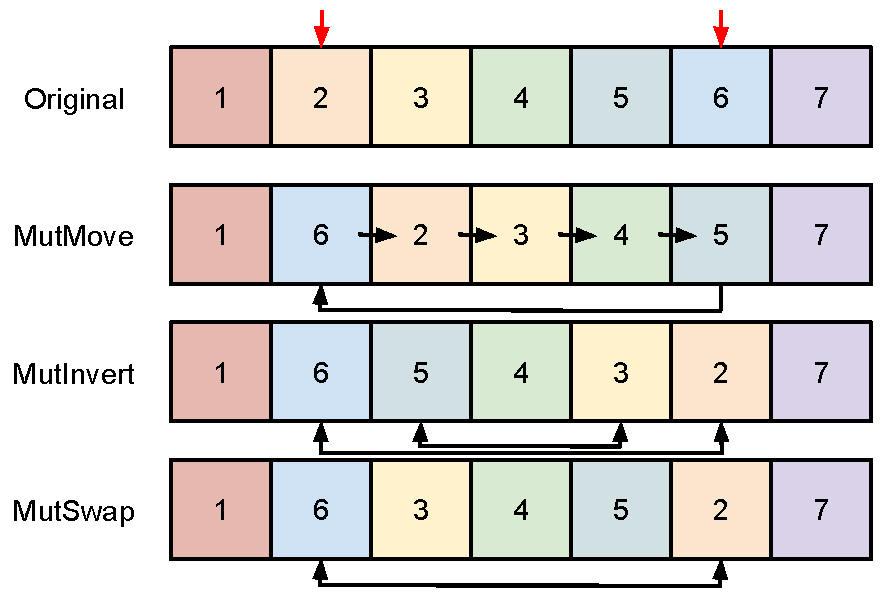
\includegraphics[width=0.7\textwidth]{Figures/mutation.pdf}
  \caption{Mutationsverfahren}\label{fig.mutation}
\end{figure}

\paragraph{mutinvert}
Beschreibung

\paragraph{Ergebnisse}
vs \emph{mutswap}

Mutationsrate bei allen 3 verschiedenen Verfahren jeweils verändert.

\lstinputlisting[language=Matlab, firstline=44, lastline=51]{Code/suite.m}

\input{Chapters/gen/Mutation.Rate.mutmove}

\input{Chapters/gen/Mutation.Rate.mutinvert}

\input{Chapters/gen/Mutation.Rate.mutswap}

\begin{figure}[!h]
\minipage{0.32\textwidth}
  \includegraphics[width=\linewidth]{Figures/gen/Mutation.Rate.mutmove.png}
  \caption{mutmove}\label{fig:mutmove}
\endminipage\hfill
\minipage{0.32\textwidth}
  \includegraphics[width=\linewidth]{Figures/gen/Mutation.Rate.mutinvert.png}
  \caption{mutinvert}\label{fig:mutinvert}
\endminipage\hfill
\minipage{0.32\textwidth}%
  \includegraphics[width=\linewidth]{Figures/gen/Mutation.Rate.mutswap.png}
  \caption{mutswap}\label{fig:mutswap}
\endminipage
\end{figure}

Alle Verfahren performen ähnlich gut, daher fällt es schwer eine eindeutige
Auswahl zu treffen.
Für die optimale Parameterkonfiguration entscheiden wir uns für
{\tt mutmove} mit einer Mutationsrate von 1,25 Mutationen pro Individuum.
